\documentclass[journal]{IEEEtran}
\usepackage[utf8]{inputenc}
\usepackage{graphicx}
\usepackage{amsmath}
\usepackage{float}
\usepackage{titlesec}
\usepackage{enumitem}
\usepackage{setspace}

\titleformat{\section}[block]{\normalfont\bfseries}{\thesection}{1em}{}
\titleformat{\subsection}[block]{\normalfont\bfseries}{\thesubsection}{1em}{}
\renewcommand{\thesection}{\arabic{section}}
\renewcommand{\thesubsection}{\arabic{section}.\arabic{subsection}}



\title{Reinforcement Learning Checkpoint - Lunar Lander}
\author{Sam Lupton, Cole Hicks}

\begin{document}

\makeatletter
\def\@maketitle{%
  \newpage
  \null
  \vskip 2em%
  \begin{center}%
    \underline{\textbf{\LARGE\@title}}\par
    \vskip 1em
    {\large
      \lineskip .5em%
      \begin{tabular}[t]{c}%
        \textbf{\@author}%
      \end{tabular}\par}%
  \end{center}%
  \vskip 1.5em}
\makeatother

\maketitle

\section{Experiments - Cole}
I have implemented a SARSA algorithm for the Lunar Lander environment, utilizing epsilon-greedy exploration. The algorithm was trained with a learning rate of 0.3, a discount factor of 0.9, and an initial epsilon value of 0.3, which decayed by a factor of 0.995 per episode. To evaluate its performance, I ran the SARSA algorithm over 10,000 episodes. The parameters used for this experiment were $\alpha = 0.01, \quad \gamma = 0.99, \quad \epsilon = 0.3, \quad \text{total\_episodes} = 10000$. I hypothesized that after 10,000 episodes, the SARSA algorithm would show noticeable improvement, as SARSA is an on-policy algorithm. This means the agent updates its Q-values based on actions it has actually taken, which would allow it to refine its policy over time. I expected that, as exploration decreased, the agent would shift towards more exploitation of the best-known actions.

\section{Experiments - Sam}

I have implemented a Q-Learning algorithm for the Lunar Lander environment, utilizing epsilon-greedy exploration. The algorithm was trained with a learning rate of 0.3, a discount factor of 0.9, and an initial epsilon value of 0.3, which decayed by a factor of 0.995 per episode. To evaluate its performance, I ran the SARSA algorithm over 10,000 episodes. The parameters used for this experiment were $\alpha = 0.01, \quad \gamma = 0.99, \quad \epsilon = 0.3, \quad \text{total\_episodes} = 10000$. Since Q-Learning is an off-policy algorithm, I expected it to perform well after many episodes. Unlike SARSA, Q-Learning updates its Q-values based on the maximum possible future reward, regardless of the actions actually taken during exploration. While I anticipated strong overall performance, I also expected the agent to occasionally take suboptimal actions, particularly early in training when exploration is higher.

\section{Results - Cole}

\begin{figure}[H]
    \centering
    \vspace{-1em}
    \includegraphics[width=0.45\textwidth]{Cole's Pictures/reward-graph.png}
    \caption{SARSA Learning Progress: Total Reward per Episode.}
    \label{fig:cole_reward}
\end{figure}

SARSA algorithm performance improves significantly with more training iterations. In particular, around 1,500 episodes, we observe a noticeable increase in total rewards per episode. This improvement is largely due to the decaying epsilon value, which allows the agent to transition from exploration to exploitation, focusing more on learned strategies rather than random actions. As the training progresses, the agent becomes more consistent in achieving higher rewards, as seen in the cumulative success rate. However, some fluctuations remain due to the stochastic nature of the environment and the limitations of SARSA in balancing exploration and exploitation optimally.

\begin{figure}[H]
    \centering
    \vspace{-1em}
    \includegraphics[width=0.45\textwidth]{Cole's Pictures/cumulative-success.png}
    \caption{SARSA Learning Progress: Total Reward per Episode.}
    \label{fig:cole_reward}
\end{figure}

The cumulative success rate increases logarithmically. Just after 10,000 episodes, we achieve a cumulative success rate of 17\%.

\section{Results - Sam}

\begin{figure}[H]
    \centering
    \vspace{-1em}
    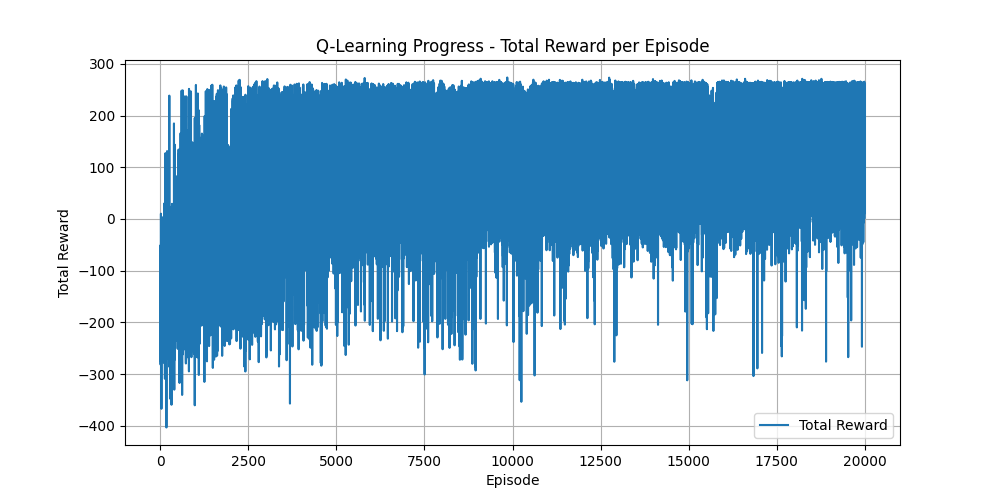
\includegraphics[width=0.45\textwidth]{Sam's Pictures/rewards_plot.png}
    \caption{Q-Learning Progress: Total Reward per Episode.}
    \label{fig:sam_rewards}
\end{figure}

The Q-Learning algorithm achieves good long-term rewards. As depicted in Figure 5, after approximately 1,500 training episodes, the reward appears to plateau, with some variation, but less frequently than in SARSA. This is because the Q-Learning algorithm, through its epsilon-greedy approach, focuses more on exploiting learned actions over time, reducing exploration. Consequently, the agent becomes more consistent in its decision-making, leading to a stabilization in rewards. However, small fluctuations remain due to the inherent stochasticity of the environment.

\begin{figure}[H]
    \centering
    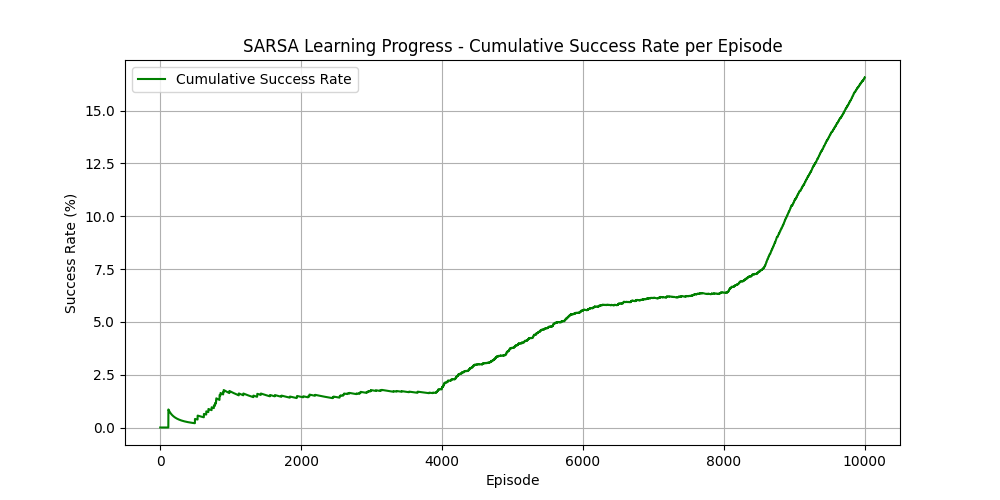
\includegraphics[width=0.45\textwidth]{Sam's Pictures/success_rate_plot.png}
    \caption{Q-Learning Progress: Cumulative Success Rate per Episode.}
    \label{fig:sam_success}
\end{figure}

The cumulative success rate increases logarithmically. Just after 10,000 episodes, we achieve a cumulative success rate of 35\%, with a significant portion of the successes occurring in the last 5,000 episodes.

\section{Difficulties - Cole}

In the beginning, it was difficult to understand that SARSA works on-policy compared to things like Q-Learning where it is off-policy, so I had to figure out how to program this. Also, testing the Lunar Lander was very time consuming, especially when there are a lot of iterations (like 20,000). Another difficulty I faced and am still facing, is tuning the hyper-parameters. It is challenging to balance everything for long-term learning when there are a lot of episodes, versus modifying for testing purposes where the iterations are decreased run more experiments.

\section{Difficulties - Sam}

While developing the Q-Learning algorithm, I encountered several challenges. Understanding the algorithm itself was one hurdle, but implementing it proved to be even more difficult due to its complexity. Testing the algorithm also presented additional challenges. However, using print statements for debugging helped identify issues. Additionally, testing involved a lot of trial and error. Experimenting with different gamma values, for example, gave me a deeper understanding of how the algorithm works and how it responds to changes in parameters. Over time, these adjustments allowed me to refine the algorithm and improve its performance.

\section{To-Do - Cole}

\begin{enumerate}[label=\arabic*.]
    \item Optimize the current SARSA implementation to improve its cumulative success rate and learning stability. Experiment with increasing the number of discretization bins, adjusting the learning rate $\alpha$, and modifying the epsilon decay rate. I also want to experiment with the number of episodes for testing. As explained above, I ran SARSA for 10,000 episodes, but I think it will be beneficial for trying out various iterations of the program.
    \item Implement eligibility traces for the SARSA algorithm (SARSA($\lambda$)) to enhance learning by crediting past actions. I also want to experiment with the parameters in this algorithm to optimize the learning of the Lunar Lander.
\end{enumerate}

\section{To-Do - Sam}
\begin{enumerate}[label=\arabic*.]
    \item Optimize the current Q-Learning implementation to enhance its cumulative success rate and reduce reward fluctuations. Experiment with increasing the number of discretization bins, adjusting the learning rate $\alpha$, and modifying the epsilon decay rate. I also want to experiment with the number of episodes for testing. As explained above, I ran Q-Learning for 10,000 episodes, but I think it will be beneficial for trying out various iterations of the program to align with the TD-Learning framework.
    \item Implement the Monte Carlo method with epsilon-greedy exploration, averaging returns over full episodes to update Q-values. I also want to experiment with the parameters in this algorithm to optimize the learning of the Lunar Lander and compare its performance to the optimized Q-Learning implementation.
\end{enumerate}
\end{document}Sam's Pictures/}